\FloatBarrier
\Needspace{12\baselineskip}
\section{Evaluation and results}
\label{sec:evaluation}
The evaluation examines two kinds of improvement: how manuscripts change through sustained revision, and what results research strategies achieve after evolution. Rating-change prediction is tested separately to assess whether the feedback component can identify changes following existing author responses.

\FloatBarrier
\subsection{Evaluation protocol: attempts, manuscripts, and passes}
\label{sec:protocol}
After inspecting the archive, we selected G0 initialization and three generations of evolution, G1--G3, as the reporting window. The archive also contains later generations. This window records 64 research attempts, 630 research invocations, 28 completed manuscripts, and 15 model-assessment passes for the best retained versions. Failed attempts and attempts without completed manuscripts remain in the totals.\src{10}

\begin{table}[H]
\centering\small
\begin{tabularx}{\textwidth}{P{43mm}Y}
\toprule
\rowcolor{warm}
\textbf{Unit or definition} & \textbf{Meaning in this report}\\
\midrule
Research attempt (episode) & A complete research execution; failures enter totals and invocation counts\\
Research invocation & A launch of the research-stage executor recorded by the historical driver\\
Completed manuscript & The required manuscript artifacts were produced; completion is counted separately from passing review\\
Current-round pass & The version under review in that round meets the historical Accept rule\\
Best retained-version pass & Uses the assessment labels of the restored version with the highest mean score\\
Fixed inner-loop subset & The same 28 completed manuscripts, tracked through initial assessment and three revisions\\
Strategy comparison batch & Four research attempts for each initial or selected strategy in a generation\\
\bottomrule
\end{tabularx}
\caption{Units and version definitions in the mathematical evaluation. Completion, current-round passes, and retained-version passes answer distinct questions.}
\label{tab:protocol}
\end{table}

\Sub{Historical assessment and version restoration}
Each historical assessment round starts three fresh Codex sessions to evaluate a manuscript using a simulated SAC scale. At least one Accept vote counts as a pass. Initial assessment is followed by three rounds of revision and reassessment. The version with the highest mean score is then restored, along with its assessment labels. A pass here refers to the historical model-assessment rule. Real conference acceptance and the current portable version's fixed final review are separate outcomes.

Manuscript revision tracks only the 28 completed manuscripts. Failed and unfinished attempts remain in the outer-loop statistics. Each generation's initial and selected strategy batches contain four attempts each. In G0 and G1, the two roles refer to the same batch, which is counted only once in the overall ledger.

\Sub{Strategy comparison and invocation coverage}
Historical strategies select specific targets from a supplied direction, so comparisons reflect both target choice and execution. The batches are adaptive, unpaired historical runs. They did not preselect identical propositions, impose equal token, dollar, or human-time budgets, or include ablations of evolutionary operators. We report counts for the selected strategies, full populations, and entire window separately, making both strategy adoption and strategy search visible.

The invocation ledger covers research-stage launches, independent review sessions, and revision attempts inferred from assessment rounds after the initial one. Each review group contains three independent sessions. Totals count sessions; group counts are not added again. The combined invocation count is a cost proxy. It does not cover strategy coaching and breeding, internal model and tool calls, unrecorded retries, full billed tokens, dollars, or active human time.

\Sub{Process evidence and prediction metrics}
Idea-screening case E1 comes from early staged reassessment. The two-round rebuttal record uses a historical internal proxy's stopping rule. These records show changes in execution decisions. Rating prediction instead uses existing papers, reviews, and responses, with labels given by the sign of final minus initial ratings. The mathematical statistics can be checked against public aggregate data; prediction metrics retain the source report's values. The evaluation protocol accompanies the report.

\FloatBarrier
\subsection{Manuscript revision: current passes rise from 3 to 12}
\label{sec:inner-results}
The same 28 completed manuscripts undergo initial assessment and three revisions. Current-version passes are 3, 10, 10, and 12, while mean scores rise from about 4.65 to 5.67. Figure~\ref{fig:inner} shows the current-version trajectory. Table~\ref{tab:rounds} also reports the best versions retained through each round.

\Fig{\earfigure{inner_progress}}{The fixed subset of 28 manuscripts from G0--G3. Current-version passes and mean scores are shown for initial assessment and three revisions. Best retained-version results appear in Table~\ref{tab:rounds}.}{fig:inner}

\begin{table}[H]
\centering\small
\begin{tabularx}{\textwidth}{P{25mm}YYYY}
\toprule
\rowcolor{warm}
\textbf{Round} & \textbf{Current passes} & \textbf{Current mean} & \textbf{Retained passes} & \textbf{Retained mean}\\
\midrule
Initial & 3 & 4.648 & 3 & 4.648\\
Revision 1 & 10 & 5.247 & 10 & 5.270\\
Revision 2 & 10 & 5.498 & 12 & 5.568\\
Revision 3 & 12 & 5.675 & 15 & 5.790\\
\bottomrule
\end{tabularx}
\caption{Round-by-round results for the fixed manuscript subset, with 28 manuscripts in every round. Means are recomputed from recorded score sums and displayed to three decimal places; full aggregate values are included in the released data. Retained columns refer to the best versions through each round.}
\label{tab:rounds}
\end{table}

The current-version pass proportion increases from $3/28=10.7\%$ to $12/28=42.9\%$, with an initial-to-final mean-score gain of about 1.03. Relative to initial assessment, 27 manuscripts improve in mean score at the last round and one declines. Model assessments of this subset improve overall after revision. The records lack a reassessment-only control, however, so they do not isolate the causal benefit of feedback-guided revision.\src{10}

\Sub{Keep the highest-scoring version when revision regresses}
Version trajectories also include regressions. Thirteen manuscripts have lower means in the last round than at their own historical best. Three have a passing best version but a non-passing last version. Restoring the highest-mean versions yields 15 retained passes, compared with 12 current passes at the final round. These regressions illustrate the practical role of version history: revision can continue while an earlier, stronger manuscript remains available for delivery.

\FloatBarrier
\subsection{Selected G3 strategy: more passes, fewer invocations}
\label{sec:strategy-results}
Figure~\ref{fig:evolution} reports the historical pass rate of each generation's selected strategy. Each point represents four complete research attempts, including failed and unfinished attempts in the denominator. The selected batches in G0 and G1 have no passes; G2 has $2/4$ and G3 has $3/4$. Each generation uses its own selected strategy and research targets.

\Fig{\earfigure{evolution_progress}}{Selected-strategy pass rates for G0 initialization and G1--G3 are 0\%, 0\%, 50\%, and 75\%. Each point represents four historical research attempts, rather than repeated measurement of one strategy on fixed tasks.}{fig:evolution}

\Sub{Turn the last episode's problems into the next strategy's changes}
The outer loop brings exit reasons and review comments into strategy revision. Recorded changes include shortening candidate lists, requesting core lemmas and proof routes earlier, and raising contribution requirements. Subsequent batches test those changes through research outcomes. Table~\ref{tab:strategy-batches} gives the initial and selected strategy counts; Table~\ref{tab:population} gives the full population ledger.

\begin{table}[H]
\centering\small
\begin{tabularx}{\textwidth}{P{13mm}YYYY}
\toprule
\rowcolor{warm}
\textbf{Gen.} & \textbf{Initial passes / attempts} & \textbf{Selected passes / attempts} & \textbf{Initial research invocations} & \textbf{Selected research invocations}\\
\midrule
G0 & 0/4 & 0/4 & 53 & 53\\
G1 & 0/4 & 0/4 & 40 & 40\\
G2 & 0/4 & 2/4 & 24 & 45\\
G3 & 2/4 & 3/4 & 41 & 29\\
\bottomrule
\end{tabularx}
\caption{Historical batch comparison of the initial strategy and each generation's selected strategy. In G0 and G1, both roles refer to the same batch and cannot be counted twice in the full population.}
\label{tab:strategy-batches}
\end{table}

\begin{table}[H]
\centering\small
\begin{tabularx}{\textwidth}{P{14mm}YYYYY}
\toprule
\rowcolor{warm}
\textbf{Gen.} & \textbf{Attempts} & \textbf{Research invocations} & \textbf{Completed papers} & \textbf{Retained passes} & \textbf{Pass rate}\\
\midrule
G0 & 12 & 169 & 1 & 0 & 0.0\%\\
G1 & 16 & 155 & 5 & 1 & 6.25\%\\
G2 & 16 & 148 & 8 & 5 & 31.25\%\\
G3 & 20 & 158 & 14 & 9 & 45.0\%\\
\midrule
Total & 64 & 630 & 28 & 15 & 23.4\%\\
\bottomrule
\end{tabularx}
\caption{Full G0--G3 population counts. Failed and unfinished attempts remain in the denominator. Selected batches and population-wide performance are reported separately; retained passes use the best-version rule.}
\label{tab:population}
\end{table}

The G3 selected strategy passes 75\% of attempts ($3/4$), compared with 50\% ($2/4$) for the initial strategy. Counting all candidates and the initial strategy gives a G3 population rate of 45\% ($9/20$) and an overall window rate of $15/64=23.4\%$. Restricting the denominator to completed manuscripts gives $15/28=53.6\%$. These scopes distinguish adopting a selected strategy, conducting strategy search, and assessing completed manuscripts.

\Sub{Research invocations per pass fall by 52.8\%}
Both G3 strategy batches perform four research attempts. The initial strategy uses 41 research invocations and obtains two passes; the selected strategy uses 29 and obtains three. Figure~\ref{fig:cost} and Table~\ref{tab:cost} put research, review, and inferred revision in a common ledger.

\begin{figure}[H]
\centering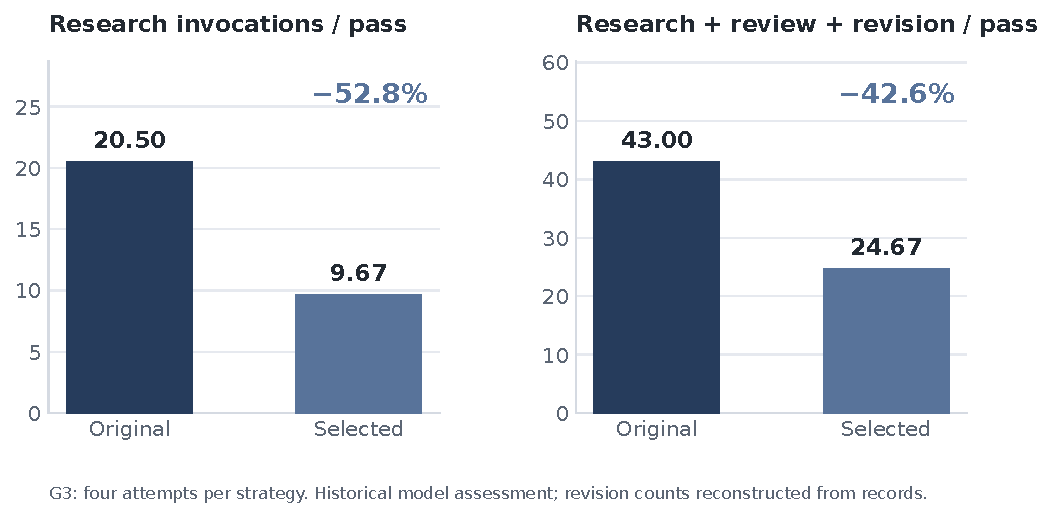
\includegraphics[width=.96\textwidth]{../../figures/en/cost_comparison.pdf}
\caption{In G3, research invocations per pass fall from $41/2=20.50$ to $29/3=9.67$, a 52.8\% reduction. The combined research, review, and inferred-revision proxy falls from $86/2=43.00$ to $74/3=24.67$, a 42.6\% reduction.}
\label{fig:cost}
\end{figure}

\begin{table}[H]
\centering\small\setlength{\tabcolsep}{3pt}
\begin{tabularx}{\textwidth}{P{22mm}rrrrrY}
\toprule
\rowcolor{warm}
\textbf{G3 strategy} & \textbf{Research} & \textbf{Review} & \textbf{Revision$^*$} & \textbf{Total} & \textbf{Passes} & \textbf{Total / pass}\\
\midrule
Initial & 41 & 36 & 9 & 86 & 2 & 43.00\\
Selected & 29 & 36 & 9 & 74 & 3 & 24.67\\
\bottomrule
\end{tabularx}
\caption{G3 invocation ledger, with four attempts per batch. Each batch has 12 review groups and 36 independent sessions. Revision$^*$ is inferred from assessment rounds after the initial one; review groups are not added again to the session total.}
\label{tab:cost}
\end{table}

Research invocations per attempt fall from $41/4=10.25$ to $29/4=7.25$, while passes increase from two to three. Together these produce the 52.8\% reduction in research invocations per pass. Including review and inferred revision gives a 42.6\% reduction in the combined proxy per pass. Section~\ref{sec:protocol} defines both scopes; full machine costs and human time are not included.

Counting the entire search process, G0--G3 use 630 research invocations for 15 passes, or 42 research invocations per pass. This ledger includes the investment in finding strategies and is reported separately from the cost of adopting the G3 selected batch. Invocations per pass are undefined for batches with zero passes.

\Sub{The pass definition changes the comparison}
We also apply a stricter diagnostic to the retained review votes: all three votes must be Accept, and each score must be at least 7. Both the G3 initial and selected strategies satisfy this requirement in only $1/4$ attempts. No new reviews were run. This diagnostic shows how the historical pass rule affects the interpretation of the advantage. Small batches, self-selected targets, and a reporting window chosen after inspecting the archive also limit generalization. Stable benefits require matched tasks, consistent quality checks, and full resource accounting.\src{10}

\FloatBarrier
\Needspace{180mm}
\subsection{Rating prediction: stronger on rises and ties, weaker on falls}
\label{sec:rebuttal-results}
The rebuttal feedback evaluator reads a paper, its initial review, and the author's recorded response, then predicts whether the rating rises, stays unchanged, or falls. Each case is supplied separately. The final rating is used only to check the label, with actual change given by $\operatorname{sign}(R_{\mathrm{final}}-R_{\mathrm{initial}})$.

The test joins public OpenReview historical records with ProReviewer initial ratings. It uses DeepSeek V4 Pro, isolated cases, zero-shot prompting, and temperature 0. Table~\ref{tab:rebuttal-eval} reports aggregate results from the source report. Macro-F1 averages the F1 scores across classes; higher values, up to 1, are better.\src{1,8,10}

\begin{table}[H]
\centering\small
\begin{tabularx}{\textwidth}{P{39mm}Y P{18mm}}
\toprule
\rowcolor{warm}
\textbf{Source and sample} & \textbf{Prediction setting} & \textbf{Macro-F1}\\
\midrule
36-case balanced subset & 18 rises and 18 unchanged ratings; excludes falls & 0.805\\
57-case full test & Rise, no change, and fall; includes six falls & 0.503\\
Same 57-case source set & Source-reported rise/no-change metric$^*$ & 0.755\\
\bottomrule
\end{tabularx}
\caption{Prediction of post-response rating changes. $^*$The third row comes from the same 57-case source set, but its effective binary denominator was not reported separately. The rows use different evaluation settings. F1 values are retained from the source; public materials do not include per-case predictions for reestimation.}
\label{tab:rebuttal-eval}
\end{table}

The balanced binary test yields a Macro-F1 of 0.805; the full three-class test yields 0.503, with F1 of 0 for the falling-rating class. Detecting falls is a clear weakness of this evaluator, which the binary test does not cover. Further prompt changes did not improve held-out performance, so the original zero-shot prompt was retained. Model weights were not changed.

EAR combines rating-change predictions with evidence checks to compare drafts. The current test asks whether rating changes can be predicted following existing responses. Whether newly generated responses improve real reviewer ratings requires a separate experiment. Response decisions still require evidence, content checks, and author judgment, particularly given the evaluator's weak detection of falling ratings.

\Sub{Public materials and result verification}
Released counts, score sums, and the evaluation protocol allow readers to check means, proportions, invocation totals, and cost per pass. Anonymous process records preserve specific turns where evidence changed a decision or feedback changed a strategy. The public aggregates do not include individual research targets, complete manuscripts, per-vote review text, per-case rebuttal predictions, or full execution logs. They support statistical checks; reproducing the complete research process requires those additional materials.
